\documentclass[13pt,dvipsnames,ignorenonframetext,aspectratio = 1610]{beamer}
\setbeamertemplate{caption}[numbered]
\setbeamertemplate{caption label separator}{: }
\setbeamercolor{caption name}{fg=normal text.fg}
\beamertemplatenavigationsymbolsempty
\usepackage{lmodern}
\usepackage{amssymb,amsmath}
% packages
\usepackage{amsfonts, algorithm, algpseudocode, dsfont,
	pgfplots, tikz, tikzscale, ulem, xcolor}
\usetikzlibrary{arrows,shapes,positioning,external}
\pgfplotsset{compat=1.15}

\usepackage{ifxetex,ifluatex}
\usepackage{fixltx2e} % provides \textsubscript
\ifnum 0\ifxetex 1\fi\ifluatex 1\fi=0 % if pdftex
  \usepackage[T1]{fontenc}
  \usepackage[utf8]{inputenc}
\else % if luatex or xelatex
  \ifxetex
    \usepackage{mathspec}
  \else
    \usepackage{fontspec}
  \fi
  \defaultfontfeatures{Ligatures=TeX,Scale=MatchLowercase}
    \setmainfont[]{Roboto Light}
    \setmonofont[Mapping=tex-ansi]{Roboto Mono}
\fi
\usefonttheme{serif} % use mainfont rather than sansfont for slide text
% use upquote if available, for straight quotes in verbatim environments
\IfFileExists{upquote.sty}{\usepackage{upquote}}{}
% use microtype if available
\IfFileExists{microtype.sty}{%
\usepackage{microtype}
\UseMicrotypeSet[protrusion]{basicmath} % disable protrusion for tt fonts
}{}
\newif\ifbibliography
\hypersetup{
            pdftitle={Linear Regression, Priors, and Model Selection},
            pdfauthor={Jon Fintzi},
            colorlinks=true,
            linkcolor=Maroon,
            citecolor=Blue,
            urlcolor=red,
            breaklinks=true}
%\urlstyle{same}  % Use monospace font for urls

% Prevent slide breaks in the middle of a paragraph:
\widowpenalties 1 10000
\raggedbottom

\AtBeginPart{
  \let\insertpartnumber\relax
  \let\partname\relax
  \frame{\partpage}
}
\AtBeginSection{
  \ifbibliography
  \else
    \let\insertsectionnumber\relax
    \let\sectionname\relax
    \frame{\sectionpage}
  \fi
}
\AtBeginSubsection{
  \let\insertsubsectionnumber\relax
  \let\subsectionname\relax
  \frame{\subsectionpage}
}

\setlength{\parindent}{0pt}
\setlength{\parskip}{6pt plus 2pt minus 1pt}
\setlength{\emergencystretch}{3em}  % prevent overfull lines
\providecommand{\tightlist}{%
  \setlength{\itemsep}{0pt}\setlength{\parskip}{0pt}}
\setcounter{secnumdepth}{0}


\title[Linear Regression, Priors, and Model Selection]{Linear Regression, Priors, and Model Selection}
\author[
Jon Fintzi
]{Jon Fintzi}
\institute[
Biostatistics Research Branch
]{
Biostatistics Research Branch \\
National Institute of Allergy and Infectious Diseases\\
National Institutes of Health
}
\date[
09/08/19
]{
September 08, 2019
}

% ------------------------------------------------------------------------------------------------
% BELOW ARE MY ADDITIONS
% ------------------------------------------------------------------------------------------------

% ------------------------------------------------------------------------------------------------
% CUSTOM COMMANDS
% ------------------------------------------------------------------------------------------------
\newcommand{\Var}{\mathrm{Var}}
\newcommand{\E}{\mathrm{E}}
\newcommand{\expit}{\mathrm{expit}}
\newcommand{\logit}{\mathrm{logit}}
\newcommand{\mr}[1]{\mathrm{#1}}
\newcommand{\mb}[1]{\mathbf{#1}}
\newcommand{\mi}[1]{\mathit{#1}}
\newcommand{\bs}[1]{\boldsymbol{#1}}
\newcommand{\rmd}{\mr{d}}
\newcommand{\ind}[1]{\mathds{1}_{\left \lbrace#1\right \rbrace}}
\newcommand{\deriv}[2]{\frac{\rmd#1}{\rmd#2}}
\newcommand{\pdiv}[2]{\frac{\partial#1}{\partial#2}}
\newcommand{\diag}{\mr{diag}}
\newcommand{\wtil}[1]{\widetilde{#1}}
\newcommand{\what}[1]{\widehat{#1}}

\newcommand{\shrug}[1][]{%
	\begin{tikzpicture}[baseline,x=0.8\ht\strutbox,y=0.8\ht\strutbox,line width=0.125ex,#1]
	\def\arm{(-2.5,0.95) to (-2,0.95) (-1.9,1) to (-1.5,0) (-1.35,0) to (-0.8,0)};
	\draw \arm;
	\draw[xscale=-1] \arm;
	\def\headpart{(0.6,0) arc[start angle=-40, end angle=40,x radius=0.6,y radius=0.8]};
	\draw \headpart;
	\draw[xscale=-1] \headpart;
	\def\eye{(-0.075,0.15) .. controls (0.02,0) .. (0.075,-0.15)};
	\draw[shift={(-0.3,0.8)}] \eye;
	\draw[shift={(0,0.85)}] \eye;
	% draw mouth
	\draw (-0.1,0.2) to [out=15,in=-100] (0.4,0.95); 
\end{tikzpicture}}
% ------------------------------------------------------------------------------------------------
%	PACKAGE LIST
% ------------------------------------------------------------------------------------------------
\usepackage{
booktabs,
%fontspec,
graphicx,
multicol,
pgfplots,
ragged2e,
tabularx,
wasysym,
hyperref,
hanging,
multirow,
eso-pic,
}

\usepackage[export]{adjustbox}
% ------------------------------------------------------------------------------------------------
%	GRAPHICS PATH
% ------------------------------------------------------------------------------------------------
\graphicspath{{./figs/}}


% ------------------------------------------------------------------------------------------------
%	TABLE OF CONTENTS
% ------------------------------------------------------------------------------------------------
\useoutertheme[subsection=false,shadow]{miniframes}
\setbeamertemplate{section in toc}[sections numbered]
\setbeamertemplate{subsection in toc}[subsections numbered]

% ------------------------------------------------------------------------------------------------
%	ITEMIZE
% ------------------------------------------------------------------------------------------------
\setbeamertemplate{itemize item}{$\bullet$}
\setbeamertemplate{itemize subitem}{$\circ$}
\setbeamertemplate{itemize subsubitem}{$\bullet$}

\setlength{\parskip}{0.5em}

% ------------------------------------------------------------------------------------------------
%	COLORS
% ------------------------------------------------------------------------------------------------

% sthlm Colors
\definecolor{sthlmLightBlue}{RGB}{0,91,150}
\definecolor{sthlmBlue}{RGB}{3,57,108}
\definecolor{sthlmDarkBlue}{RGB}{1,31,75}
\definecolor{sthlmLightRed}{RGB}{143,39,39}
\definecolor{sthlmRed}{RGB}{124,0,0}
\definecolor{sthlmLightYellow}{RGB}{255,204,0}
\definecolor{sthlmYellow}{RGB}{255,149,0}
\definecolor{sthlmPurple}{RGB}{64,0,64}
\definecolor{sthlmGreen}{RGB}{25,77,51}
\definecolor{sthlmGrey}{RGB}{142,142,147}
\definecolor{sthlmLightGrey}{RGB}{233,233,233}
\definecolor{sthlmDarkGrey}{RGB}{61,61,70}

% General
\setbeamercolor{normal text}{fg=sthlmDarkGrey}
\hypersetup{colorlinks=true, urlcolor=sthlmDarkBlue, linkcolor=sthlmDarkGrey, citecolor=sthlmDarkBlue}
\setbeamercolor{structure}{fg=sthlmDarkGrey}
\setbeamercolor{alerted text}{fg=sthlmRed}
\setbeamercolor{example text}{fg=white}
\setbeamercolor{copyright text}{fg=sthlmLightBlue}
\setbeamercolor{palette primary}{fg=sthlmDarkGrey}
\setbeamercolor{palette secondary}{fg=sthlmDarkGrey,bg=sthlmLightGrey}
\setbeamercolor{palette tertiary}{fg=black,bg=sthlmDarkGrey}
\setbeamercolor{palette quaternary}{fg=white, bg=sthlmDarkGrey}

\setbeamercolor{mini frame}{bg=sthlmLightGrey}
\setbeamercolor{section in head/foot}{fg=sthlmDarkGrey, bg=sthlmLightGrey}

% Titlepage
\setbeamercolor{title}{parent=normal text}
\setbeamercolor{subtitle}{parent=normal text}
\setbeamercolor{institute}{parent=normal text}

% Content
\setbeamercolor{frametitle}{parent=palette quaternary}

% Blocks
\setbeamercolor{block title}{fg=white,bg=sthlmBlue}
\setbeamercolor{block body}{fg=sthlmDarkGrey, bg=sthlmLightGrey}
\setbeamercolor{block title example}{fg=white, bg=sthlmGreen}
\setbeamercolor{block body example}{fg=sthlmDarkGrey, bg=sthlmLightGrey}
\setbeamercolor{block title alerted}{fg=white, bg=sthlmLightRed}
\setbeamercolor{block body alerted}{fg=sthlmDarkGrey, bg=sthlmLightGrey}

% Notes
\setbeamercolor{note page}{fg=sthlmDarkGrey,bg=sthlmLightGrey}
\setbeamercolor{note title}{fg=white, bg=sthlmDarkGrey}
\setbeamercolor{note date}{parent=note title}

% Page Number
\setbeamercolor{page number in head/foot}{fg=sthlmDarkGrey}

\setbeamercolor{qed}{fg=sthlmGrey}
\setbeamercolor{itemize item}{fg=sthlmDarkBlue}
\setbeamercolor{itemize subitem}{fg=sthlmDarkBlue}
\setbeamercolor{itemize subsubitem}{fg=sthlmDarkBlue}

% ------------------------------------------------------------------------------------------------
%	FONTS
% ------------------------------------------------------------------------------------------------

% General

%% Declare fontfamilys
%\if@doNoFlama%
%	% Sans serif math option
%	\if@doSans%
%	% Sans serif math
%		\usepackage{fontspec}%
%		\setmainfont{Arial Regular}%
%	\else%
%		% Serif math
%		\usefonttheme{professionalfonts}%
%		\usepackage[no-math]{fontspec}%
%	\fi%
%	
%	\newfontfamily\Light{Arial Regular}%
%	\newfontfamily\Book{Arial Black Regular}%
%	\newfontfamily\bfseries{Arial Bold}%
%	\setsansfont{Arial Regular}%
%\else%
%	% Sans serif math option
%	\if@doSans%
%	% Sans serif math
%		\usepackage{fontspec}%
%		\setmainfont{FlamaLight}%
%	\else%
%		% Serif math
%		\usefonttheme{professionalfonts}%
%		\usepackage[no-math]{fontspec}%
%	\fi%
%	
%	\newfontfamily\Light{FlamaLight}%
%	\newfontfamily\Book{FlamaBook}%
%	\newfontfamily\bfseries{FlamaMedium}%
%	\setsansfont{FlamaLight}%
%	%\newfontfamily\texttt{SourceCodePro-Light}
%\fi%
%
%%\renewcommand\UrlFont{\texttt}
%
%% Font sizes
%
%% Titlepage
%\setbeamerfont{title}{family=\bfseries,size=\fontsize{24}{26}}
%\setbeamerfont{subtitle}{family=\Light,size=\fontsize{14}{18}}
%\setbeamerfont{subtitle}{size=\fontsize{14}{18}}
%\setbeamerfont{date}{size=\fontsize{9}{11}}
%\setbeamerfont{author}{family=\bfseries,size=\fontsize{13}{15}}
%\setbeamerfont{institute}{size=\fontsize{09}{10}}
%
%% Section
%\setbeamerfont{section title}{size*={39pt}{24pt}, family = \bfseries, series=\bfseries}% Content
%\setbeamerfont{frametitle}{family=\bfseries,size=\large}
%\setbeamerfont{copyright text}{family=\Light,size=\tiny}
%\setbeamerfont{block title}{family=\Book,size=\large}
%\setbeamerfont{block title alerted}{family=\Book,size=\large}
%\setbeamerfont{alerted text}{family=\bfseries}
%
%%Captions
%\setbeamerfont{caption name}{family=\Book}




%% ------------------------------------------------------------------------------------------------
%%	FONT ASSIGMENTS
%% ------------------------------------------------------------------------------------------------
%% Title Page
%\newfontfamily\Light{Roboto Light}
%\setbeamerfont{title}{size=\LARGE, series=\bfseries}
%\setbeamerfont{subtitle}{family=\Light, size=\small, shape=\normalfont}
%\setbeamerfont{date}{family=\Light, size=\footnotesize}
%\setbeamerfont{author}{size=\small, series=\bfseries}
%\setbeamerfont{institute}{family=\Light, size=\scriptsize}
%
%% Section
%\setbeamerfont{section title}{size=\Huge}
%
%% Content
%\setbeamerfont{frametitle}{size=\Large, series=\bfseries}
%\setbeamerfont{copyright text}{size=\tiny}
%\setbeamerfont{block title}{size=\large, series=\bfseries}
%\setbeamerfont{block title alerted}{size=\large, series=\bfseries}
%\setbeamerfont{block title example}{size=\large, series=\bfseries}
%
%\setbeamerfont{caption}{size=\small}
%\setbeamerfont{caption name}{family=\small}

% ------------------------------------------------------------------------------------------------
%	FONT ASSIGMENTS
% ------------------------------------------------------------------------------------------------
% Title Page
%\newfontfamily\Light{Roboto Light}
\setbeamerfont{title}{size=\LARGE, series=\bfseries}
\setbeamerfont{subtitle}{size=\normalsize, shape=\normalfont}
\setbeamerfont{date}{size=\normalsize}
\setbeamerfont{author}{size=\normalsize, series=\bfseries}
\setbeamerfont{institute}{size=\small}

% Section
\setbeamerfont{section title}{size=\Huge}

% Content
\setbeamerfont{frametitle}{size=\Large, series=\bfseries}
\setbeamerfont{copyright text}{size=\tiny}
\setbeamerfont{block title}{size=\large, series=\bfseries}
\setbeamerfont{block title alerted}{size=\large, series=\bfseries}
\setbeamerfont{block title example}{size=\large, series=\bfseries}

\setbeamerfont{caption}{size=\small}
\setbeamerfont{caption name}{family=\small}

% ------------------------------------------------------------------------------------------------
%	TITLE PAGE
% ------------------------------------------------------------------------------------------------

\newcommand\AtPageUpperRight[1]{\AtPageUpperLeft{%
 \put(\LenToUnit{\paperwidth},\LenToUnit{0\paperheight}){#1}%
 }}%
\newcommand\AtPageLowerRight[1]{\AtPageLowerLeft{%
 \put(\LenToUnit{\paperwidth},\LenToUnit{0\paperheight}){#1}%
 }}%

%\AddToShipoutPictureBG*{% Add picture to current page
%  \AtStockLowerLeft{% Add picture to lower-left corner of paper stock
%    \includegraphics[width=\stockwidth,height=\stockheight]{tiger}}% http://latex.tug.org/texlive/devsrc/Master/texmf-dist/doc/generic/pstricks/images/tiger.eps
%}

% Titlepage structure
\def\maketitle{\ifbeamer@inframe\titlepage\else\frame[plain]{\titlepage}\fi}
\def\titlepage{\usebeamertemplate{title page}}
\setbeamertemplate{title page}
%\frame[plain]{\titlepage}
{
	% Add background to title page
  	%\AddToShipoutPictureFG*{\includegraphics[width=\paperwidth]{backgroundiegs.pdf}}
	%\AddToShipoutPictureFG*{
	%	\AtPageLowerRight{\put(-95, 0){
	%		\includegraphics[width=.2\paperwidth]{title_graphic.pdf}}}}
	%\AddToShipoutPictureFG*{\includegraphics[width=\paperwidth]{youngmetro_logo.png}}
	\begin{minipage}[b][\paperheight]{\textwidth}
	%\vspace*{5mm}
	%\includegraphics[height=14mm]{./logo}\par
	\vspace*{20mm}
	\ifx\insertsubtitle\@empty%
	\else%
		{\usebeamerfont{title}\usebeamercolor[fg]{title}\MakeUppercase{\inserttitle}\parskip0pt\par}%
	\fi%
	\ifx\insertsubtitle\@empty%
	\else%
		{\usebeamerfont{subtitle}\usebeamercolor[fg]{subtitle}\insertsubtitle\par}%
		\vspace*{5mm}
	\fi%
	\ifx\insertdate\@empty%
	\else%
		{\usebeamerfont{date}\usebeamercolor[fg]{date}\insertdate\par}%
	\fi% 
	
	\vfill
	
	\ifx\insertauthor\@empty%
	\else%
		{\usebeamerfont{author}\usebeamercolor[fg]{author}\insertauthor\par}%
	\fi%
	\ifx\insertinstitut\@empty%
	\else%
		\vspace*{1mm}
		{\usebeamerfont{institute}\usebeamercolor[sthlmDarkGrey]{institute}\insertinstitute\par}%
	\fi% 
	\vspace*{5mm}
	\end{minipage}
}

% ------------------------------------------------------------------------------------------------
%	SECTION PAGES
% ------------------------------------------------------------------------------------------------

% Make Sectionhead uppercase
\newcommand{\insertsectionHEAD}{%
	\expandafter\insertsectionHEADaux\insertsectionhead}
	\newcommand{\insertsectionHEADaux}[3]{\MakeUppercase{#3}
}

\if@doSectionPage\@empty
\else
% Insert frame with section title at every section start
\AtBeginSection[]
{
\begingroup
\setbeamercolor{background canvas}{bg=sthlmDarkGrey}
\begin{frame}[plain]
\centering
\vfill\usebeamerfont{section title}\textcolor{white}{\insertsectionHEAD}\vfill
\end{frame}
\endgroup
}
\fi

% ------------------------------------------------------------------------------------------------
%	HEADLINE
% ------------------------------------------------------------------------------------------------
\makeatletter
\def\progressbar@progressbar{} % the progress bar
\newcount\progressbar@tmpcounta% auxiliary counter
\newcount\progressbar@tmpcountb% auxiliary counter
\newdimen\progressbar@pbht %progressbar height
\newdimen\progressbar@pbwd %progressbar width
\newdimen\progressbar@tmpdim % auxiliary dimension

\progressbar@pbwd=\paperwidth
\progressbar@pbht=1.25ex

% the progress bar
\def\progressbar@progressbar{%
    \progressbar@tmpcounta=\insertframenumber
    \progressbar@tmpcountb=\inserttotalframenumber
    \progressbar@tmpdim=\progressbar@pbwd
%    \divide\progressbar@tmpdim by 100
%    \multiply\progressbar@tmpdim by \progressbar@tmpcounta
%    \divide\progressbar@tmpdim by \progressbar@tmpcountb
%    \multiply\progressbar@tmpdim by 100
  \begin{tikzpicture}[very thin]

    \shade[top color=sthlmLightGrey,bottom color=sthlmLightGrey,middle color=sthlmLightGrey]
      (0pt, 0pt) rectangle ++ (\progressbar@pbwd, \progressbar@pbht);

      \shade[draw=sthlmDarkBlue,top color=sthlmDarkBlue,bottom color=sthlmDarkBlue,middle color=sthlmDarkBlue] %
        (0pt, 0pt) rectangle ++ (\progressbar@tmpdim, \progressbar@pbht);

  \end{tikzpicture}%
}

\setbeamertemplate{headline}{

  \begin{beamercolorbox}[wd=\paperwidth,ht=1ex,center,dp=0ex]{sthlmLightGrey}%
    \progressbar@progressbar%
  \end{beamercolorbox}%
}

%% ------------------------------------------------------------------------------------------------
%%	FRAME TITLE IN ALL CAPS (MAC: USE "? + ? + }" to uncomment section
%% ------------------------------------------------------------------------------------------------
%\setbeamertemplate{frametitle}
%{
%\begin{beamercolorbox}[wd=\paperwidth,leftskip=0.3cm,rightskip=0.3cm,ht=3ex,dp=1.5ex]{frametitle}
%	 \usebeamerfont{frametitle}\MakeUppercase{\insertframetitle}%
%\end{beamercolorbox}
%}

% ------------------------------------------------------------------------------------------------
%	FRAME TITLE IN TITLE CASE (MAC: USE "? + ? + {" to comment-out section
% ------------------------------------------------------------------------------------------------
\setbeamertemplate{frametitle}
{
\begin{beamercolorbox}[sep=0ex,wd=\paperwidth,leftskip=0.25cm,rightskip=0.3cm,ht=2.75ex,dp=1.375ex]{frametitle}
	 \usebeamerfont*{frametitle}{\insertframetitle}%
\end{beamercolorbox}
}


%\setbeamertemplate{block alerted begin}
%{
%  \setbeamercolor{item}{parent=block body alerted}
%  \par\vskip\medskipamount%
%  \begin{beamercolorbox}[sep=.5ex,dp=0.6ex,leftskip=0.5ex,rightskip=0.5ex]{block title alerted}
%    \usebeamerfont*{block title alerted}\insertblocktitle%
%  \end{beamercolorbox}%
%  {\parskip0pt\par}%
%  {\nointerlineskip\vskip-0.5pt}%
%  \usebeamerfont{block body alerted}%
%  \begin{beamercolorbox}[sep=.5ex,dp=0.6ex,leftskip=0.5ex,rightskip=0.5ex,vmode]{block body alerted}%
%}
%\setbeamertemplate{block alerted end}
%{\end{beamercolorbox}\vskip\smallskipamount}

% ------------------------------------------------------------------------------------------------
%	FOOTLINE
% ------------------------------------------------------------------------------------------------
\usenavigationsymbolstemplate{}
\setbeamertemplate{footline}
{
  \leavevmode%
  \hbox{%
  \begin{beamercolorbox}[sep=0.25ex,wd=.333333\paperwidth,ht=3.25ex,dp=1.25ex,left]{author in head/foot}%
    \usebeamerfont{author in head/foot}\insertshortauthor\expandafter\beamer@ifempty\expandafter{\beamer@shortinstitute}{}{~~--- \insertshortinstitute}
  \end{beamercolorbox}%
  \begin{beamercolorbox}[sep=0.5ex,wd=.333333\paperwidth,ht=3.25ex,dp=1.25ex,center]{title in head/foot}%
    \usebeamerfont{title in head/foot}\insertshorttitle
  \end{beamercolorbox}%
  \begin{beamercolorbox}[sep=0.5ex,wd=.333333\paperwidth,ht=3.25ex,dp=1.25ex,right]{date in head/foot}%
    %\usebeamerfont{date in head/foot}\insertshortdate{}\hspace*{2em}
    Page \insertframenumber{} %/ \inserttotalframenumber\hspace*{2ex} 
  \end{beamercolorbox}}%
  \vskip0pt%
}

% ------------------------------------------------------------------------------------------------
%	CAPTIONS
% ------------------------------------------------------------------------------------------------
\setbeamertemplate{caption label separator}{: }

% ------------------------------------------------------------------------------------------------
%	BLOCKS
% ------------------------------------------------------------------------------------------------
\setbeamertemplate{block begin}
{
  \setbeamercolor{item}{parent=block body}
  \par\vskip\medskipamount%
  \begin{beamercolorbox}[sep=.5ex,dp=0.6ex,leftskip=0.5ex,rightskip=0.5ex]{block title}
    \usebeamerfont*{block title}\insertblocktitle%
  \end{beamercolorbox}%
  {\parskip0pt\par}%
  {\nointerlineskip\vskip-0.5pt}%
  \usebeamerfont{block body}%
  \begin{beamercolorbox}[sep=.5ex,dp=0.6ex,leftskip=0.5ex,rightskip=0.5ex,vmode]{block body}%
}
\setbeamertemplate{block end}  
{\end{beamercolorbox}\vskip\smallskipamount}

\setbeamertemplate{block alerted begin}
{
  \setbeamercolor{item}{parent=block body alerted}
  \par\vskip\medskipamount%
  \begin{beamercolorbox}[sep=.5ex,dp=0.6ex,leftskip=0.5ex,rightskip=0.5ex]{block title alerted}
    \usebeamerfont*{block title alerted}\insertblocktitle%
  \end{beamercolorbox}%
  {\parskip0pt\par}%
  {\nointerlineskip\vskip-0.5pt}%
  \usebeamerfont{block body alerted}%
  \begin{beamercolorbox}[sep=.5ex,dp=0.6ex,leftskip=0.5ex,rightskip=0.5ex,vmode]{block body alerted}%
}
\setbeamertemplate{block alerted end}
{\end{beamercolorbox}\vskip\smallskipamount}

\setbeamertemplate{block example begin}
{
  \par\vskip\medskipamount%
  \begin{beamercolorbox}[sep=.5ex,dp=0.6ex,leftskip=0.5ex,rightskip=0.5ex]{block title example}
    \usebeamerfont*{block title example}\insertblocktitle%
  \end{beamercolorbox}%
  {\parskip0pt\par}%
  {\nointerlineskip\vskip-0.5pt}%
  \usebeamerfont{block body example}%
  \begin{beamercolorbox}[sep=.5ex,dp=0.6ex,leftskip=0.5ex,rightskip=0.5ex,vmode]{block body example}%
}
\setbeamertemplate{block example end}
{\end{beamercolorbox}\vskip\smallskipamount}

% ------------------------------------------------------------------------------------------------
%	BLOCK HOVERING ABOVE THE SLIDE
% ------------------------------------------------------------------------------------------------

\newcommand<>{\hover}[1]{\uncover#2{%
	\begin{tikzpicture}[remember picture,overlay]%
	\draw[fill,opacity=0.4] (current page.south west)
	rectangle (current page.north east);
	\node at (current page.center) {#1};
	\end{tikzpicture}}
	}

% ------------------------------------------------------------------------------------------------
%	VERTICALLY ALIGNED COLUMNS
% ------------------------------------------------------------------------------------------------
	
\usepackage{environ}% Required for \NewEnviron, i.e. to read the whole body of the environment

\newcounter{acolumn}%  Number of current column
\newlength{\acolumnmaxheight}%   Maximum column height


% `column` replacement to measure height
\newenvironment{@acolumn}[1]{%
    \stepcounter{acolumn}%
    \begin{lrbox}{\@tempboxa}%
    \begin{minipage}{#1}%
}{%
    \end{minipage}
    \end{lrbox}
    \@tempdimc=\dimexpr\ht\@tempboxa+\dp\@tempboxa\relax
    % Save height of this column:
    \expandafter\xdef\csname acolumn@height@\roman{acolumn}\endcsname{\the\@tempdimc}%
    % Save maximum height
    \ifdim\@tempdimc>\acolumnmaxheight
        \global\acolumnmaxheight=\@tempdimc
    \fi
}

% `column` wrapper which sets the height beforehand
\newenvironment{@@acolumn}[1]{%
    \stepcounter{acolumn}%
    % The \autoheight macro contains a \vspace macro with the maximum height minus the natural column height
    \edef\autoheight{\noexpand\vspace*{\dimexpr\acolumnmaxheight-\csname acolumn@height@\roman{acolumn}\endcsname\relax}}%
    % Call original `column`:
    \orig@column{#1}%
}{%
    \endorig@column
}

% Save orignal `column` environment away
\let\orig@column\column
\let\endorig@column\endcolumn

% `columns` variant with automatic height adjustment
\NewEnviron{acolumns}[1][]{%
    % Init vars:
    \setcounter{acolumn}{0}%
    \setlength{\acolumnmaxheight}{0pt}%
    \def\autoheight{\vspace*{0pt}}%
    % Set `column` environment to special measuring environment
    \let\column\@acolumn
    \let\endcolumn\end@acolumn
    \BODY% measure heights
    % Reset counter for second processing round
    \setcounter{acolumn}{0}%
    % Set `column` environment to wrapper
    \let\column\@@acolumn
    \let\endcolumn\end@@acolumn
    % Finally process columns now for real
    \begin{columns}[#1]%
        \BODY
    \end{columns}%
}

% ------------------------------------------------------------------------------------------------
%	IMAGES
% ------------------------------------------------------------------------------------------------

\newbox\mytempbox
\newdimen\mytempdimen

\newcommand\includegraphicscopyright[3][]{%
  \leavevmode\vbox{\vskip3pt\raggedright\setbox\mytempbox=\hbox{\includegraphics[#1]{#2}}%
    \mytempdimen=\wd\mytempbox\box\mytempbox\par\vskip1pt%
    \usebeamerfont{copyright text}{\usebeamercolor[fg]{copyright text}{\vbox{\hsize=\mytempdimen#3}}}\vskip3pt%
}}

\begin{document}

% Hide progress bar and footline on titlepage
\begin{frame}[plain]
\titlepage
\end{frame}

\begin{frame}{Dead and Company are Playing in Hampton, VA on 11/8}
\protect\hypertarget{dead-and-company-are-playing-in-hampton-va-on-118}{}

\textbf{Nothing like Bayesian modeling to make you feel alive!} Last
time, we talked about: \vspace{-0.1in}

\begin{itemize}
\tightlist
\item
  Bayesian inference \emph{always} starts with a model for the
  \textbf{joint distribution} of \(\theta\) and \(y\):.\vspace{-0.1in}
  \[\pi(\theta, y) = f(y|\theta)\pi(\theta) = \pi(\theta|y)m(y).\vspace{-0.1in}\]
\item
  \textbf{Bayes rule} yields the \textbf{posterior distribution}
  \vspace{-0.1in}
  \[\pi(\theta|y) =  \frac{f(y,\theta)}{m(y)} = \frac{f(y|\theta)\pi(\theta)}{m(y)} \propto Likelihood\times Prior.\vspace{-0.1in}\].
\item
  All of the information used in the \emph{update} to our prior is
  encoded in the \textbf{likelihood},\vspace{-0.1in}
  \[L(\mb{y}|\theta) = \prod_{i=1}^N f(y_i|y_{1,\dots,i-1}\theta).\vspace{-0.1in}\]
\item
  Re-Analysis of PREVAIL II data with non-conjugate priors:

  \begin{itemize}
  \tightlist
  \item
    Prior distributions for geometric mean log odds of 28 day mortality
    and ratio of the odds of death in 28 days for ZMapp vs.~oSOC.\\
  \item
    Posteriors are distributions of these \emph{parameters} given the
    data, updated under binomial likelihood.
  \item
    First look at \texttt{Stan}.
  \end{itemize}
\end{itemize}

\end{frame}

\begin{frame}{Lectures 3-4 of Statistical Rethinking}
\protect\hypertarget{lectures-3-4-of-statistical-rethinking}{}

Briefly:

\begin{itemize}
\tightlist
\item
  Probability statements that describe key aspects of the data
  generating mechanism.
\item
  Language for modeling: \vspace{-0.1in} \begin{align*}
    y_i &\sim \mr{N}(\mu_i,\sigma^2), \\
    \mu_i &= \beta_0 + \beta_1 x_{i,1} + \beta_p x_{i,p}, \\ 
    \beta &\sim \mr{N}(0,10^2), \\ 
    \sigma &\sim \mr{Exponential}(1), \\
    x_i &\sim \mr{N}(0,1).
  \end{align*}
\item
  Here, the prior is full of lines, so too is the posterior is full of
  lines.
\item
  Nothing special about lines, e.g., could use polynomials, splines,
  etc. Nothing special about linearity either.
\item
  Bayesian framework takes a generative model with lots of uncertainty
  as input, learns which configurations of parameters are consonant with
  the data, and returns a generative model with (hopefully) less
  uncertainty.
\end{itemize}

\end{frame}

\begin{frame}{Common Hangups}
\protect\hypertarget{common-hangups}{}

Probably the two most common hangups are

\begin{enumerate}
\tightlist
\item
  How to choose priors? What happens if the priors are ``wrong''?
\item
  Small world model, big world data.
\end{enumerate}

Today, we'll talk about

\begin{enumerate}
\tightlist
\item
  How the shape or a prior affects the posterior.
\item
  Some principles for prior selection.
\item
  Good practices for workflow as they relate to model building and
  validation.
\end{enumerate}

\end{frame}

\begin{frame}{Example - Linear Regression for Height vs.~Weight}
\protect\hypertarget{example---linear-regression-for-height-vs.weight}{}

(Similar to Statistical Rethinking, lecture 3) Suppose we want to
understand how height predicts weight in a sample of 241 adult women.

\begin{itemize}
\tightlist
\item
  Simulate:
  \(h_i = 150 + 0.55 w_i + \epsilon_i,\ \epsilon_i\sim N(0,4.5^2).\)
\item
  Straightforward, probably won't matter much what we do.
\end{itemize}

\begin{center}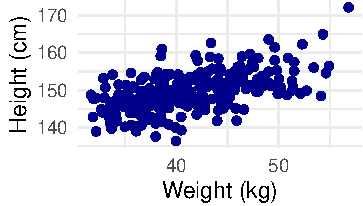
\includegraphics{linreg_priors_files/figure-beamer/ht_wt_plot1-1} \end{center}

\end{frame}

\begin{frame}{Example - Linear Regression for Height vs.~Weight}
\protect\hypertarget{example---linear-regression-for-height-vs.weight-1}{}

Model with ``non-informative'' priors\footnote<.->{Stupid priors.}:

\[\begin{aligned}
h_i &\sim Normal(\mu_i, \sigma^2)\\ 
\mu_i &= \alpha + \beta(w_i - \bar{w}) \\
\alpha &\sim Normal(160, 160^2) \\
\beta &\sim Normal(0, 100^2) \\
\sigma &\sim Half-Cauchy(10)
\end{aligned}\]

I'll fit this using the \texttt{brms} package, which generates
\texttt{Stan} code, compiles, and fits the model. Take a look at the raw
Rmarkdown file if you're interested in seeing the code.

\end{frame}

\begin{frame}{Example - Linear Regression for Height vs.~Weight}
\protect\hypertarget{example---linear-regression-for-height-vs.weight-2}{}

Prior predictive draws are clearly absurd, but it's a really simple
model with a fair amount of data so let's just pretend to not care.

\begin{figure}

{\centering 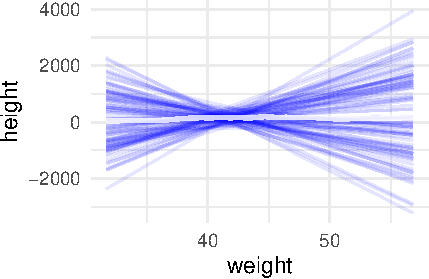
\includegraphics{linreg_priors_files/figure-beamer/ht_wt_priorpred_stupid-1} 

}

\caption{Prior distribution}\label{fig:ht_wt_priorpred_stupid}
\end{figure}

\end{frame}

\begin{frame}{Example - Linear Regression for Height vs.~Weight}
\protect\hypertarget{example---linear-regression-for-height-vs.weight-3}{}

But, the posterior seems to shake out OK.

\begin{figure}

{\centering 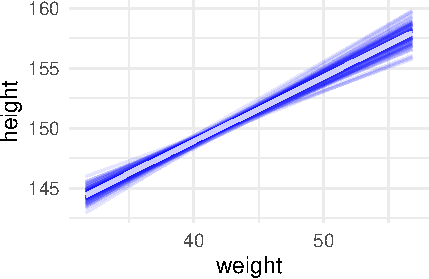
\includegraphics{linreg_priors_files/figure-beamer/ht_wt_post_me-1} 

}

\caption{Posterior distribution of regression lines.}\label{fig:ht_wt_post_me}
\end{figure}

\end{frame}

\begin{frame}{Example - Linear Regression for Height vs.~Weight}
\protect\hypertarget{example---linear-regression-for-height-vs.weight-4}{}

Posterior distributions of model parameters seem reasonable and credible
intervals contain the true values.

\begin{figure}

{\centering 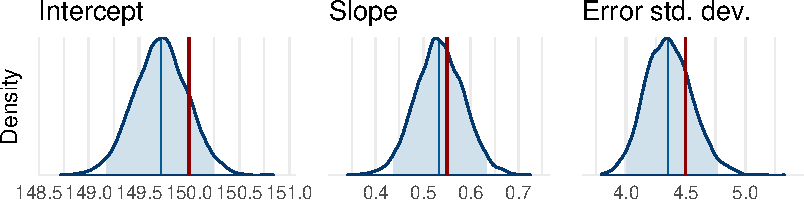
\includegraphics{linreg_priors_files/figure-beamer/ht_wt_post_stupid-1} 

}

\caption{Parameter posteriors and 95 percent credible intervals.}\label{fig:ht_wt_post_stupid}
\end{figure}

\end{frame}

\begin{frame}{Example - Linear Regression for Height vs.~Weight}
\protect\hypertarget{example---linear-regression-for-height-vs.weight-5}{}

Observed data are contained within the posterior predictive
distributions.

\begin{figure}

{\centering 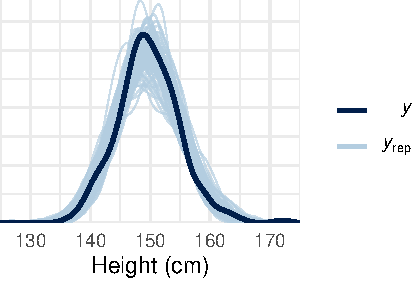
\includegraphics{linreg_priors_files/figure-beamer/ht_wt_stupid_postpred-1} 

}

\caption{Density plots of observed heights and draws from the posterior predictive distribution.}\label{fig:ht_wt_stupid_postpred}
\end{figure}

\end{frame}

\begin{frame}{Example - Linear Regression for Height vs.~Weight}
\protect\hypertarget{example---linear-regression-for-height-vs.weight-6}{}

Leave-one-out posterior predictive distributions (\texttt{loo} package,
more
\href{https://avehtari.github.io/modelselection/}{\textcolor{red}{here}})
indicate good predictive performance.

\begin{figure}

{\centering 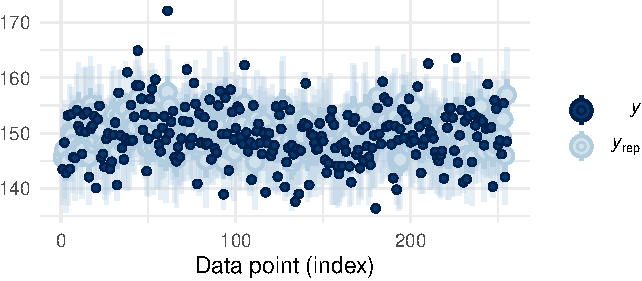
\includegraphics{linreg_priors_files/figure-beamer/ht_wt_stupid_postpred_loo-1} 

}

\caption{Observed heights and leave-one-out 95 percent posterior predictive intervals.}\label{fig:ht_wt_stupid_postpred_loo}
\end{figure}

\end{frame}

\begin{frame}{We Escaped the Zombies but They Ate the Dog}
\protect\hypertarget{we-escaped-the-zombies-but-they-ate-the-dog}{}

In this case, we had a lot of data to estimate a fairly strong signal.

\emph{Bernstein-von Mises (BvM) theorem}: under some conditions, the
posterior will look asymptotically like the sampling distribution of a
maximum likelihood estimator, i.e., multivariate normal with mean at the
true population parameter, \(\bs{\theta}_0\), and covariance matrix
\(\bs{\Sigma} = \frac{1}{n}I(\bs{\theta}_0)^{-1}\).

\begin{itemize}
\tightlist
\item
  See Section 2.2.5
  \href{http://www.statslab.cam.ac.uk/~nickl/Site/__files/stat2013.pdf}{\textcolor{red}{here}}
  for a technical discussion.
\item
  Related paper by Charlie Geyer on ``no-n'' asymptotics of MLEs,
  available
  \href{http://www.stat.umn.edu/geyer/lecam/simple.pdf}{\textcolor{red}{here}}.
\item
  Gelman 2017 (see refs) on prior selection.
\item
  From the
  \href{\%7Bhttps://en.wikipedia.org/wiki/Bernstein\%E2\%80\%93von_Mises_theorem\%7D}{\textcolor{red}{Wiki}},
  quoting A. W. F. Edwards, ``It is sometimes said\ldots{}that the
  choice of prior distribution is unimportant in practice\ldots{}when
  there are moderate amounts of data. The less said about this `defence'
  the better.''
\end{itemize}

\end{frame}

\begin{frame}{We Escaped the Zombies but They Ate the Dog}
\protect\hypertarget{we-escaped-the-zombies-but-they-ate-the-dog-1}{}

Dan Simpson summarizes the problem in an epic rant,
\href{https://statmodeling.stat.columbia.edu/2017/11/27/asymptotically-we-are-all-dead/}{\textcolor{red}{Asymptotically we're all dead}}:

\begin{itemize}
\tightlist
\item
  There are some important assumptions needed for BvM:

  \begin{enumerate}
  \tightlist
  \item
    The MLE is consistent for the true population parameter.
  \item
    The model has a fixed, finite number of parameters.
  \item
    The true parameter \(\theta_0\) lies on the interior of the
    parameter space.
  \item
    The prior must be non-zero in a neighborhood around \(\theta_0\).
  \item
    The log-likelihood must be smooth.
  \end{enumerate}
\item
  Incredibly difficult to apply BvM in practice.

  \begin{itemize}
  \tightlist
  \item
    Need independent replications of the same experiment, not enough to
    just have a lot of data.
  \item
    Assumptions unlikely to hold in settings where we'd want to use
    penalized estimators or when we have an infinite dimensional
    parameter.
  \item
    Most datasets are not instantaneous snapshots of a stationary
    process.
  \end{itemize}
\end{itemize}

\textbf{Moral of the story:} The zombies could have bitten Fido and
you'd never know until it's too late.

\end{frame}

\begin{frame}{Poorly Informed Regression}
\protect\hypertarget{poorly-informed-regression}{}

Suppose we only had height-weight measurements for 5 women instead of on
241. How will the prior affect our inferences?\vspace{-0.1in}

\begin{itemize}
\tightlist
\item
  Obviously, we expect a ton of uncertainty in the posterior. Might seem
  like a silly example, how far can we really get with only ten
  measurements?
\item
  The things that go wrong in this setting are exactly what can go wrong
  without our realizing it in more complex settings.
\item
  We are going through this exercise to understand the failure modes of
  different priors when the priors are not properly calibrated to the
  scale of the data.
\item
  When the model fails, how does it fail?
\end{itemize}

\begin{center}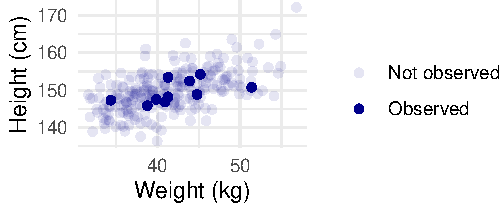
\includegraphics{linreg_priors_files/figure-beamer/plot_dat_sub-1} \end{center}

\end{frame}

\begin{frame}{Poorly Informed Regression: Analysis with
``Non-informative'' Priors}
\protect\hypertarget{poorly-informed-regression-analysis-with-non-informative-priors}{}

The posterior contains associations that don't make sense.

\begin{figure}

{\centering 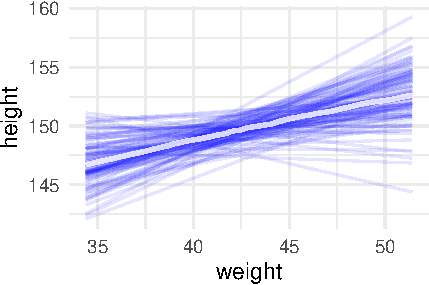
\includegraphics{linreg_priors_files/figure-beamer/ht_wt_post_me2-1} 

}

\caption{Posterior distribution of regression lines.}\label{fig:ht_wt_post_me2}
\end{figure}

\end{frame}

\begin{frame}{Poorly Informed Regression: Analysis with
``Non-informative'' Priors}
\protect\hypertarget{poorly-informed-regression-analysis-with-non-informative-priors-1}{}

Leave-one-out posterior predictive distributions (\texttt{loo} package)
indicate poor predictive performance.

\begin{figure}

{\centering 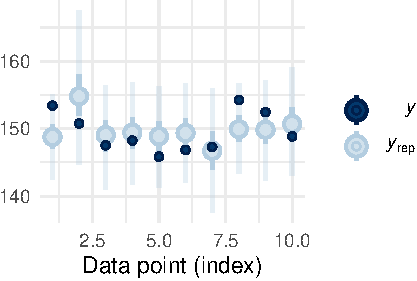
\includegraphics{linreg_priors_files/figure-beamer/ht_wt_stupid_postpred_loo2-1} 

}

\caption{Observed heights and leave-one-out 95 percent posterior predictive intervals.}\label{fig:ht_wt_stupid_postpred_loo2}
\end{figure}

\end{frame}

\begin{frame}{Poorly Informed Regression: Analysis with
``Non-informative'' Priors}
\protect\hypertarget{poorly-informed-regression-analysis-with-non-informative-priors-2}{}

\textbf{Failure mode of diffuse priors in weak data settings:}

\begin{itemize}
\tightlist
\item
  Posterior contains implausible values.
\item
  Poor predictive performance.
\end{itemize}

Uncontroversial opinions:

\begin{itemize}
\tightlist
\item
  We could have ruled out negative associations and extreme associations
  by choosing coherent priors.
\item
  We should still have a lot of uncertainty, no reason to pretend that
  we have strong information. It would be fine for the prior to be
  dominant in the posterior.
\item
  Our uncertainty should, at least, be constrained to coherent ranges
  that could plausibly have produced the data.
\item
  For more examples, see Gabry (2019).
\end{itemize}

\end{frame}

\begin{frame}{Weakly informative priors}
\protect\hypertarget{weakly-informative-priors}{}

\textbf{Basic idea:} Introduce scale information, e.g., about order of
magnitude or signs of parameters, in order to regularize inferences.

\begin{itemize}
\tightlist
\item
  Well defined units and meaningful parameterizations.
\item
  Does not necessarily leverage full domain-specific knowledge.
\item
  Requires an understanding of how the likelihood, prior, and data
  interact in the \emph{joint} model.
\item
  In our example, weakly informed prior on average height for a person
  of average weight and on slope s.t. encode a positive association and
  unlikely to observe someone more extreme than the shortest and tallest
  people in the world.
\item
  Another example, \texttt{RStanArm} puts a weakly informative prior on
  transformed parameters in linear regression via a QR decomposition of
  the design matrix, see
  \href{https://cran.r-project.org/web/packages/rstanarm/vignettes/lm.html}{\textcolor{red}{here}}.
\end{itemize}

\end{frame}

\begin{frame}{Poorly Informed Regression: Analysis with Weakly
Informative Priors}
\protect\hypertarget{poorly-informed-regression-analysis-with-weakly-informative-priors}{}

Model with weakly informative priors \footnote<.->{Be a good Bayesian
  and look some stuff up:
  \href{https://en.wikipedia.org/wiki/List_of_average_human_height_worldwide}{\textcolor{red}{height}}
  and
  \href{https://en.wikipedia.org/wiki/Human_body_weight}{\textcolor{red}{weight}}.}:

\[\begin{aligned}
h_i &\sim Normal(\mu_i, \sigma^2)\\ 
\mu_i &= \alpha + \beta(w_i - \bar{w}) \\
\alpha &\sim Normal(160, 20^2) \\
\beta &\sim LogNormal(0, 1) \\
\sigma &\sim HalfNormal(5)
\end{aligned}\]

\end{frame}

\begin{frame}{Poorly Informed Regression: Analysis with Weakly
Informative Priors}
\protect\hypertarget{poorly-informed-regression-analysis-with-weakly-informative-priors-1}{}

Prior distribution:

\begin{center}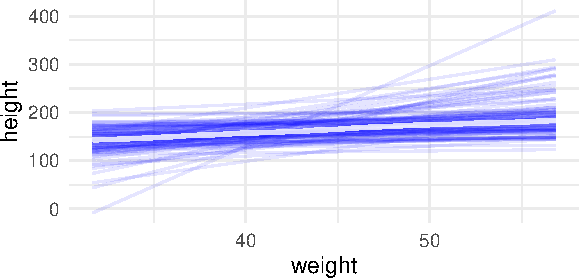
\includegraphics{linreg_priors_files/figure-beamer/ht_wt_priorfit_wi-1} \end{center}

\end{frame}

\begin{frame}{Poorly Informed Regression: Analysis with Weakly
Informative Priors}
\protect\hypertarget{poorly-informed-regression-analysis-with-weakly-informative-priors-2}{}

Much more sensible posterior.

\begin{figure}

{\centering 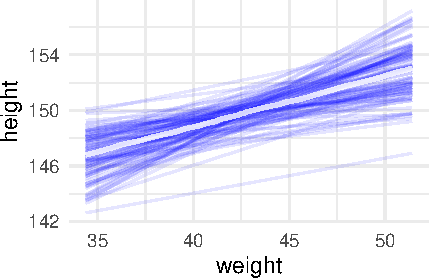
\includegraphics{linreg_priors_files/figure-beamer/ht_wt_post_me3-1} 

}

\caption{Posterior distribution of regression lines.}\label{fig:ht_wt_post_me3}
\end{figure}

\end{frame}

\begin{frame}{Poorly Informed Regression: Analysis with Weakly
Informative Priors}
\protect\hypertarget{poorly-informed-regression-analysis-with-weakly-informative-priors-3}{}

Posterior distributions of model parameters seem reasonable, not crazy
wide.

\begin{figure}

{\centering 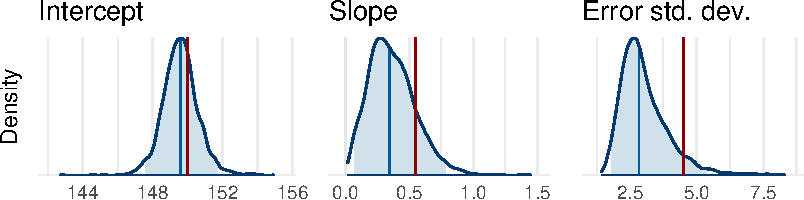
\includegraphics{linreg_priors_files/figure-beamer/ht_wt_post_wi-1} 

}

\caption{Parameter posteriors and 95 percent credible intervals.}\label{fig:ht_wt_post_wi}
\end{figure}

\end{frame}

\begin{frame}{Poorly Informed Regression: Analysis with Weakly
Informative Priors}
\protect\hypertarget{poorly-informed-regression-analysis-with-weakly-informative-priors-4}{}

Leave-one-out posterior predictive distributions are still wide, but
perform better (\(ELPD_{WI} - ELPD_{NI} \approx 0.3 \pm 0.1\)).

\begin{figure}

{\centering 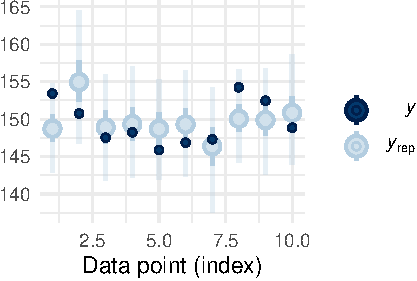
\includegraphics{linreg_priors_files/figure-beamer/ht_wt_wi_postpred_loo2-1} 

}

\caption{Observed heights and leave-one-out 95 percent posterior predictive intervals.}\label{fig:ht_wt_wi_postpred_loo2}
\end{figure}

\end{frame}

\begin{frame}{Poorly Informed Regression: Failure Mode of Light Tailed
Priors}
\protect\hypertarget{poorly-informed-regression-failure-mode-of-light-tailed-priors}{}

What if our prior is too tight and we get the location wrong?

\[\begin{aligned}
h_i &\sim Normal(\mu_i, \sigma^2)\\ 
\mu_i &= \alpha + \beta(w_i - \bar{w}) \\
\alpha &\sim Normal(170, 2.5) \\
\beta &\sim LogNormal(0, 1.25) \\
\sigma &\sim HalfNormal(5)
\end{aligned}\]

\end{frame}

\begin{frame}{Poorly Informed Regression: Failure Mode of Light Tailed
Priors}
\protect\hypertarget{poorly-informed-regression-failure-mode-of-light-tailed-priors-1}{}

Prior distribution:

\begin{center}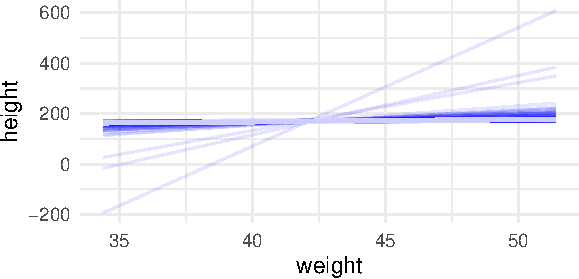
\includegraphics{linreg_priors_files/figure-beamer/ht_wt_priorfit_wi2-1} \end{center}

\end{frame}

\begin{frame}{Poorly Informed Regression: Failure Mode of Light Tailed
Priors}
\protect\hypertarget{poorly-informed-regression-failure-mode-of-light-tailed-priors-2}{}

Nothing super glaring here?

\begin{figure}

{\centering 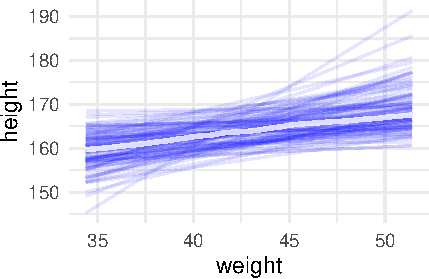
\includegraphics{linreg_priors_files/figure-beamer/ht_wt_post_me4-1} 

}

\caption{Posterior distribution of regression lines.}\label{fig:ht_wt_post_me4}
\end{figure}

\end{frame}

\begin{frame}{Poorly Informed Regression: Failure Mode of Light Tailed
Priors}
\protect\hypertarget{poorly-informed-regression-failure-mode-of-light-tailed-priors-3}{}

Ugh oh. Notice how the posterior doesn't contract relative to the prior.

\begin{figure}

{\centering 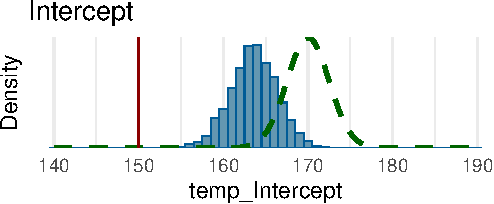
\includegraphics{linreg_priors_files/figure-beamer/ht_wt_post_wi2-1} 

}

\caption{Parameter posteriors and 95 percent credible intervals.}\label{fig:ht_wt_post_wi2}
\end{figure}

\end{frame}

\begin{frame}{Poorly Informed Regression: Failure Mode of Light Tailed
Priors}
\protect\hypertarget{poorly-informed-regression-failure-mode-of-light-tailed-priors-4}{}

Systematic bias in leave-one-out predictive densities is bad news bears!

\begin{figure}

{\centering 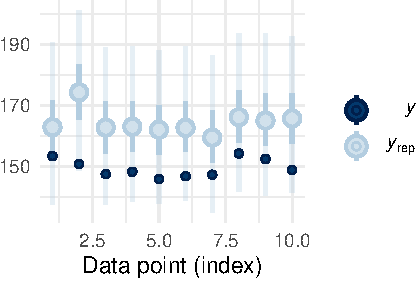
\includegraphics{linreg_priors_files/figure-beamer/ht_wt_wi_postpred_loo3-1} 

}

\caption{Observed heights and leave-one-out 95 percent posterior predictive intervals.}\label{fig:ht_wt_wi_postpred_loo3}
\end{figure}

\end{frame}

\begin{frame}{Poorly Informed Regression: Failure Mode of Heavy Tailed
Priors}
\protect\hypertarget{poorly-informed-regression-failure-mode-of-heavy-tailed-priors}{}

What if our prior is too diffuse and we get the location wrong?

\[\begin{aligned}
h_i &\sim Normal(\mu_i, \sigma^2)\\ 
\mu_i &= \alpha + \beta(w_i - \bar{w}) \\
\alpha &\sim Cauchy(170, 2.5) \\
\beta &\sim LogNormal(0, 1.25) \\
\sigma &\sim HalfNormal(5)
\end{aligned}\]

\end{frame}

\begin{frame}{Poorly Informed Regression: Failure Mode of Heavy Tailed
Priors}
\protect\hypertarget{poorly-informed-regression-failure-mode-of-heavy-tailed-priors-1}{}

Posterior now contracts around the true value, but if we were to inspect
more closely we'd see that it's also leaking mass out into the tails.

\begin{figure}

{\centering 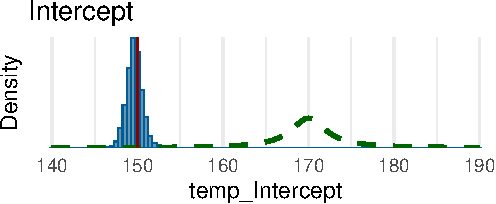
\includegraphics{linreg_priors_files/figure-beamer/ht_wt_post_wi3-1} 

}

\caption{Parameter posteriors and 95 percent credible intervals.}\label{fig:ht_wt_post_wi3}
\end{figure}

\end{frame}

\begin{frame}{Poorly Informed Regression: Failure Mode of Heavy Tailed
Priors}
\protect\hypertarget{poorly-informed-regression-failure-mode-of-heavy-tailed-priors-2}{}

Systematic bias in leave-one-out predictive densities is now gone.
Huzzah!

\begin{figure}

{\centering 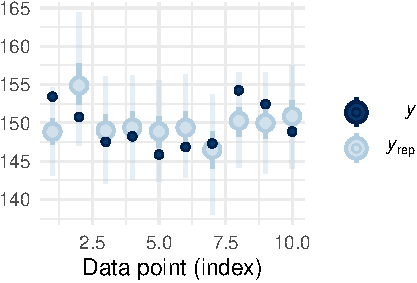
\includegraphics{linreg_priors_files/figure-beamer/ht_wt_wi_postpred_loo4-1} 

}

\caption{Observed heights and leave-one-out 95 percent posterior predictive intervals.}\label{fig:ht_wt_wi_postpred_loo4}
\end{figure}

\end{frame}

\begin{frame}{Recapping}
\protect\hypertarget{recapping}{}

Some key takeaways:

\begin{itemize}
\tightlist
\item
  We went through an iterative process to evaluate how different priors
  act on the posterior.

  \begin{enumerate}
  \tightlist
  \item
    Interrogate prior.
  \item
    Fit model.
  \item
    Criticize model.
  \item
    Wash-rinse-repeat.
  \end{enumerate}
\item
  We could have done more at each step, but we only had an hour. Read
  about robustifying Bayesian workflow
  \href{https://betanalpha.github.io/assets/case_studies/principled_bayesian_workflow.html}{\textcolor{red}{here}}.
\item
  Incorporating information about \emph{scales} can help regularize
  weakly informed models.
\item
  But remember, our goal is to identify scales that are consistent with
  our prior beliefs, not exact values.
\item
  \textbf{Big warning:} Not necessarily a good idea to look at your data
  and pick the prior to look like it. We don't know as much as we think.
  Remember, it was hubris that killed the king.
\item
  Not the only way to come up with priors, but thinking generatively
  about how parts of the model interact can help diagnose subtle issues
  that would otherwise have gone unnoticed.
\end{itemize}

\end{frame}

\begin{frame}{References}
\protect\hypertarget{references}{}

M. Betancourt ``How the Shape of a Weakly Informative Prior Affects
Inferences.''
\url{https://betanalpha.github.io/assets/case_studies/weakly_informative_shapes.html}
(2017).

J. Gabry, et al. ``Visualization in Bayesian workflow.'' \emph{Journal
of the Royal Statistical Society: Series A (Statistics in Society)}
182.2 (2019): 389-402.

A. Gelman, S. Simpson, and M. Betancourt. ``The prior can often only be
understood in the context of the likelihood.'' \emph{Entropy} 19.10
(2017): 555.

C.J. Geyer. ``Asymptotics of maximum likelihood without the LLN or CLT
or sample size going to infinity.'' \emph{Advances in Modern Statistical
Theory and Applications: A Festschrift in honor of Morris L. Eaton}.
Institute of Mathematical Statistics, 2013. 1-24.

\end{frame}

\begin{frame}{}
\protect\hypertarget{section}{}

\end{frame}

\end{document}